\documentclass[]{article}
\usepackage[a4paper]{geometry}
\renewcommand{\contentsname}{Table Of Contents}
\usepackage{amssymb}
\usepackage{hyperref}
\usepackage{fancyhdr}
\usepackage{graphicx}
\graphicspath{{./images/}}
\pagestyle{fancy}
\fancyhead{}
\fancyfoot{}
\fancyhead[L]{\slshape\MakeUppercase{Door Alarm System on Raspberry Pi 4}}
\fancyhead[R]{\slshape Angelo Barbera}
\fancyfoot[C]{\thepage}
\title{\huge Door Alarm System on Raspberry Pi 4}
\author{Angelo Barbera}
\date{2023}

\begin{document}

\begin{titlepage}
	\centering
	{\scshape\LARGE Univeristà degli Studi di Palermo \par}
	\vspace{0.6cm}
	{\scshape\Large Embedded Systems \par}
	\vspace{1.8cm}
	{\huge\bfseries Door Alarm System on Raspberry Pi 4 \par}
	\vspace{2cm}
	\vfill
	{\large Angelo Barbera 2023 \par}
\end{titlepage}

\pagenumbering{roman}

\tableofcontents

\clearpage
\pagenumbering{arabic}


\section{Introduction}
The project is a Door Alarm System. The System is able to monitor the open or closed status of a door using a hall sensor
to detect the presence of a magnet; if the latter is far from the sensor, it is emitted a sound alert with a buzzer. 
Using two LEDs and a LCD display 16x2 the status of the door is shown. In addition there is a button that can be used to 
turn off the alarm when the door is closed.
\\ 
In the following sections is described in detail the hardware and the software used to implement the project.

\section{Hardware}

\subsection{Raspberry PI 4}

\begin{center}
    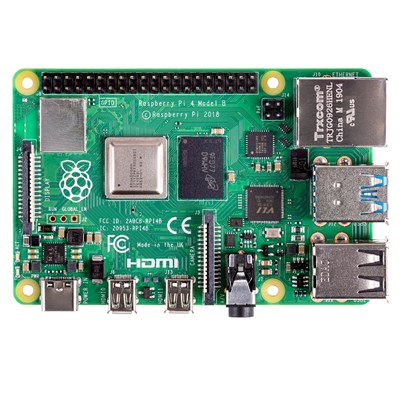
\includegraphics[scale=0.6]{raspberry_pi_4}
\end{center}
The chosen target for this project is the Raspberry Pi 4 Model B, a single board computer developed by 
the Raspberry Pi Foundation and realeased in 2019. The tech specs include:
\begin{itemize} 
    \item Broadcom BCM2711, Quad core Cortex-A72 (ARM v8) 64-bit SoC @ 1.5Ghz
    \item 1GB, 2GB, 4GB, or 8GB LPDDR4-3200 SDRAM (depending on model)
    \item 2.4 GHz and 5.0 Ghz 802.11ac wireless
    \item Gigabit Ethernet
    \item Bluetooth 5.0, BLE
    \item 2 USB 3.0 ports, 2 USB 2.0 ports
    \item Raspberry Pi standard 40 pin GPIO header
    \item 2 micro-HDMI ports (up to 4kp60 supported)
    \item 2-lane MIPI DSI display port
    \item 2-lane MIPI CSI camera port
    \item 4-pole stereo audio and composite video port
    \item H.265 (4kp60 decode), H.264 (1080p60 decode, 1080p30 encode)
    \item OpenGL ES 3.1, Vulkan 1.0
    \item Micro-SD card slot for loading operating system and data storage
    \item 5V DC via USB-C connector (minimum 3A)
    \item 5V DC via GPIO header (minimum 3A)
    \item Power over Ethernet (PoE) enabled (requires separate PoE HAT)
    \item Operating temperature 0 - 50 °C ambient
\end{itemize}

\subsection{FT232-AZ USB to TTL serial UART adapter}

\begin{center}
    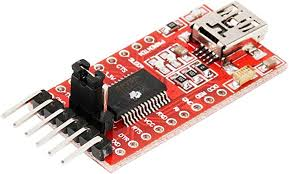
\includegraphics[scale=0.4]{uart_adapter}
\end{center}
The FT232-AZ USB to TTL serial UART adapter is used to connect the PC used during the development of the project
to the target in order to send and receive data between the PC and the Raspberry Pi 4. 
The PC is connected through a USB port, the target is connected through GPIO pins according to the 
following table.

\begin{center}
    \begin{tabular}{ |c|c|c| } 
        \hline
        GPIO & Function & UART adapter  \\
        \hline
        14 (Tx) & Output & Rx \\ 
        15 (Rx) & Input & Tx \\ 
        Ground & Ground & Ground \\ 
        \hline
    \end{tabular}
\end{center}

\subsection{KY-003 Hall sensor}

\begin{center}
    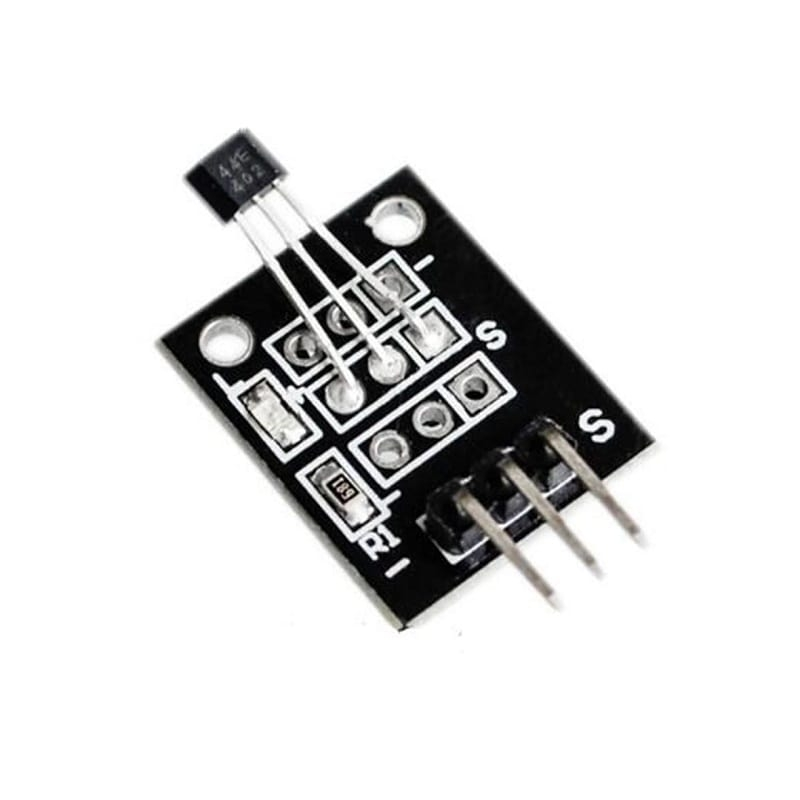
\includegraphics[scale=0.2]{ky-003}
\end{center}
The KY-003 hall sensor allows to detect a magnetic field. When the magnetic field at the Hall sensor exceeds
the operate point threshold (BOP) the output of the device switches low. When the magnetic field is reduced
to below the realease point threshold (BRP) the device output switches high.
BOP and BRP may vary respectively from 1 mT to 33 mT and from 5 mT to 35 mT at operating 
temperature T = 25° C depending on the sensor model.
This sensor is used to trigger the alarm when the magnet is far from the sensor.

\subsection{KY-012 Buzzer}

\begin{center}
    
\includegraphics[scale=0.4]{ky-012}
\end{center}
The KY-012 Buzzer is an active piezoelectric buzzer, it generates a sound of approximately 2.5kHz when 
input signal (S) is high. The Buzzer is activated when the Hall sensor does not detect the magnet.

\subsection{LEDs}

\begin{center}
    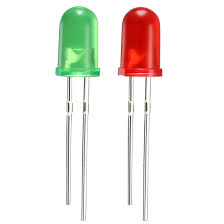
\includegraphics[scale=0.4]{leds}
\end{center}
The LEDs are used to show the alarm status. When the Hall sensor does not detects the magnet the green LED turns off 
and the red LED turns on. When the Hall sensor detect the magnet and the push button is pressed, the green LED turns on
and the red LED turns off.

\subsection{Push Button}

\begin{center}
    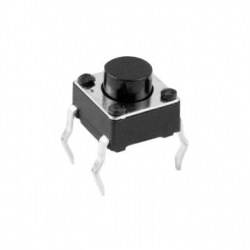
\includegraphics[scale=0.5]{push_button}
\end{center}
The push button can be used to turn off the alarm when the hall sensor detects the magnet.

\subsection{Resistors}

\begin{center}
    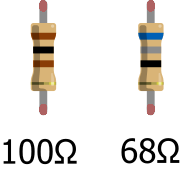
\includegraphics{resistors}
\end{center}
The resistors are connected in series to the LEDs to limit the current flowing through the LED and to ensure that the supplied 
voltage does not exceeds the maximum voltage of the LED. The 100 $ \Omega $ resistor is connected to the red LED, the 68 $ \Omega $ 
resistor is connected to the green LED.

\subsection{LCD 1602}

\begin{center}
    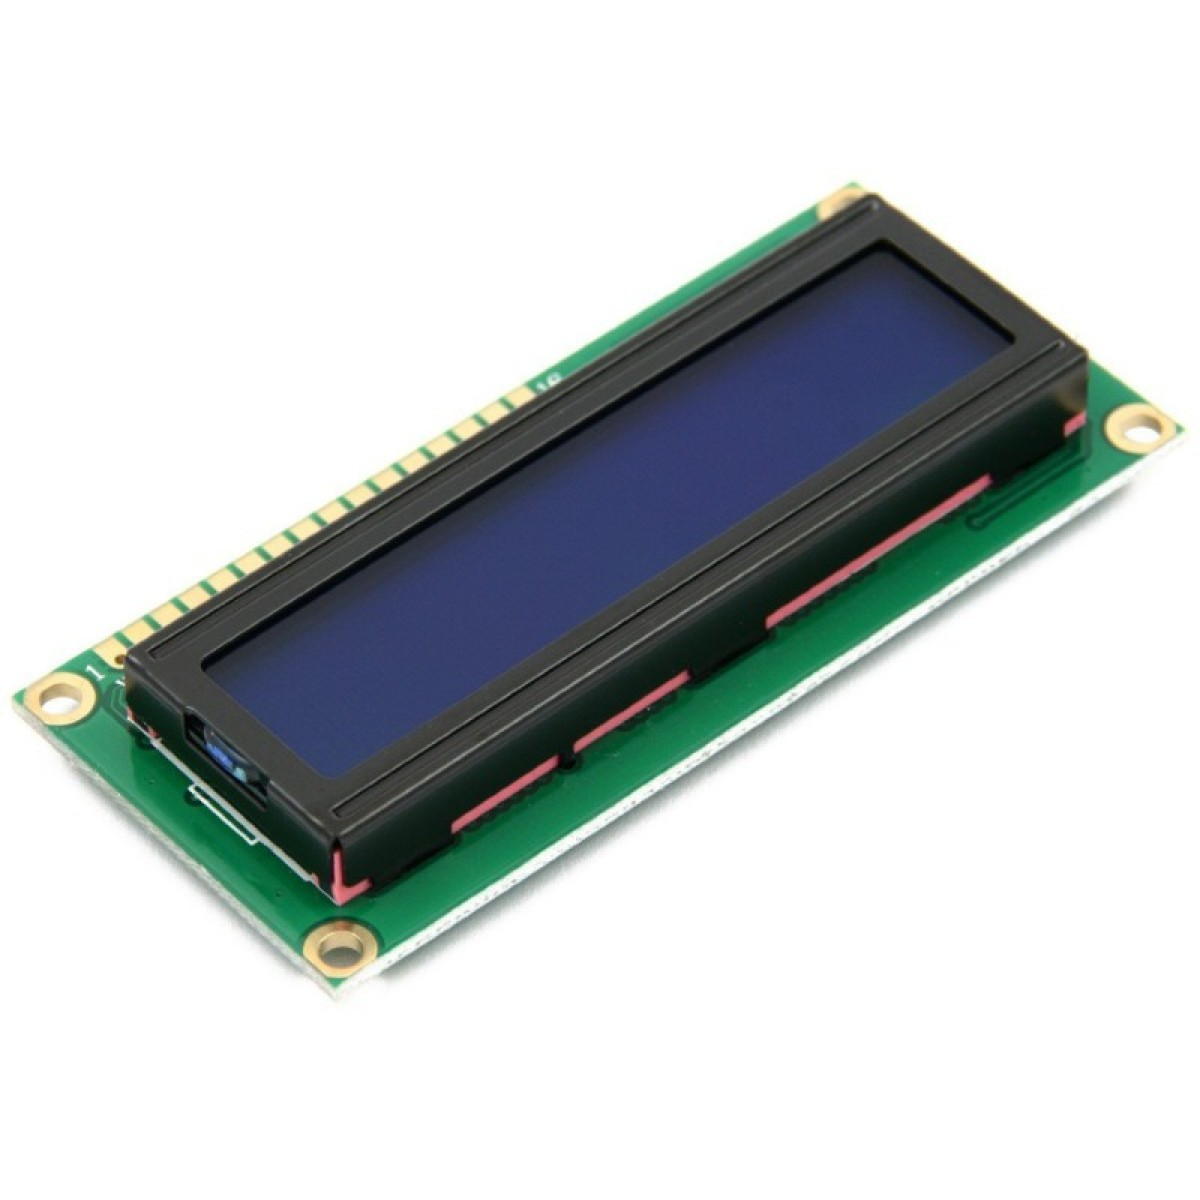
\includegraphics[scale=0.2]{lcd}
\end{center}
The LCD 1602 is an industrial character LCD that can display 16x02 or 32 characters at the same time. 
The LCD 1602 is controlled through a parrallel interface with 8-bit / 4-bit data bus and 3 control signals. 
The interface signals reach the two controller chips that drive the LCD panel as shown in the following block diagram.

\begin{center}
    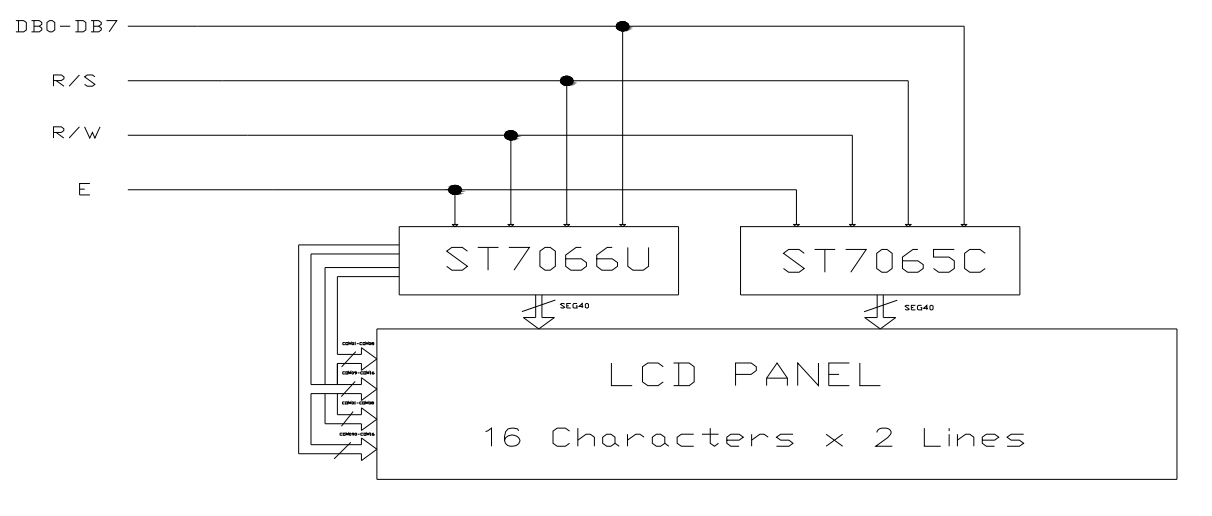
\includegraphics[scale=0.4]{lcd_block_diagram}
\end{center}
The following table describes the pin assignment

\begin{center}
    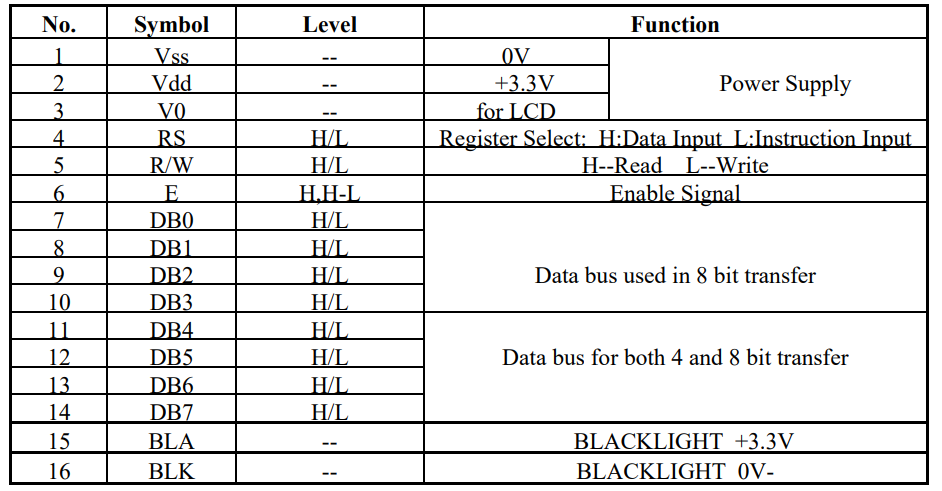
\includegraphics[scale=0.4]{lcd_pin_assignment}
\end{center}
The LCD module is controlled through instructions to set display format, data length, scrolling modality, internal RAM address, 
to perform data transfer from/to internal RAM and to access status flag. The following table describes the instructions.

\begin{center}
    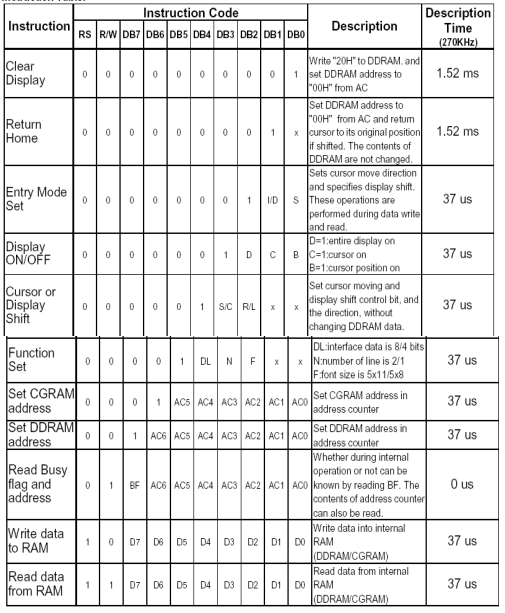
\includegraphics[scale=0.6]{lcd_instruction}
\end{center}
In order to write to the controller chips we need to set properly the control bits: the R/W bit must be set to 0 for writing,
the RS bit must be set to 1 for data input and to 0 for instruction input, the E bit must be set to 1 before the start of the data transmission
and must be set to 0 before the end of the data transmission as shown in the following figure

\begin{center}
    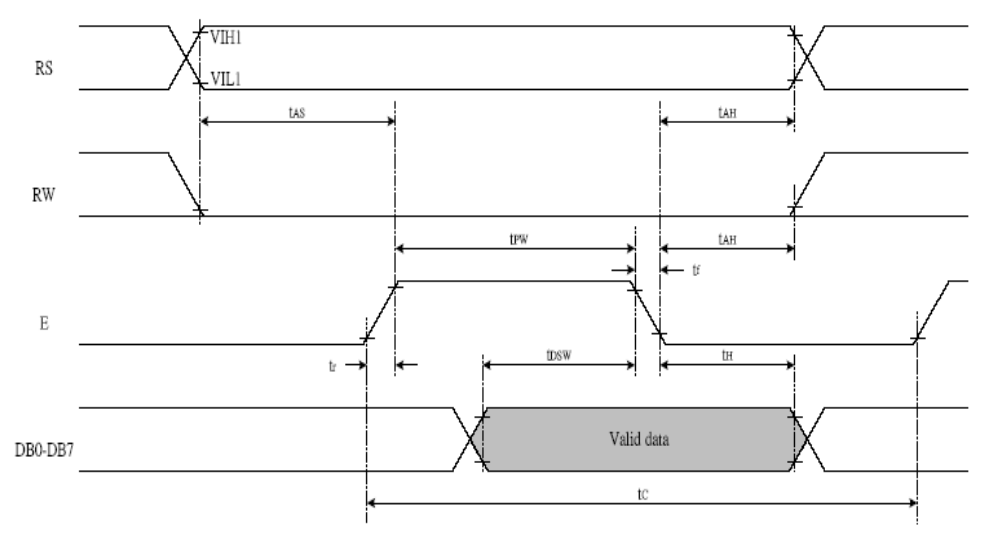
\includegraphics[scale=0.5]{lcd_writing}
\end{center}


\subsection{PCF8574AT 8-bit I/O expander for I2C bus}
\begin{center}
    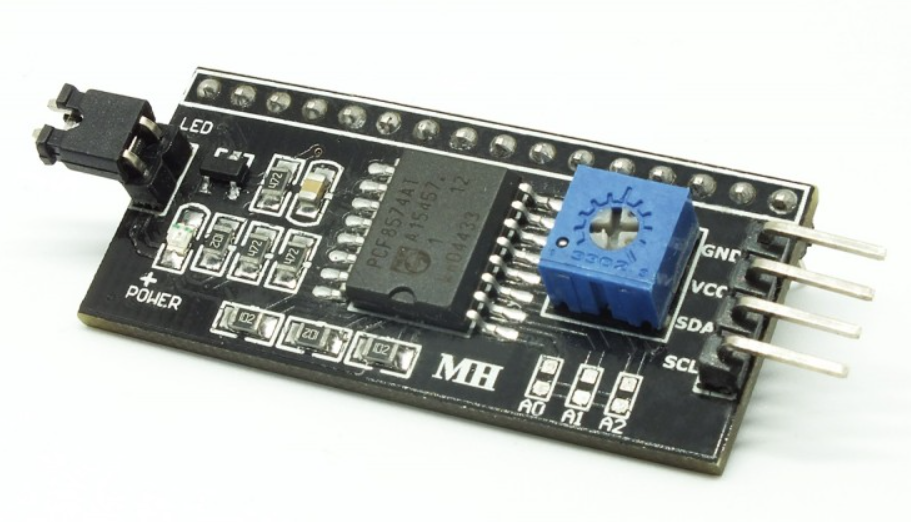
\includegraphics[scale=0.2]{io_expander}
\end{center}
The PCF8574AT provides general-purpose remote I/O expansione via the two-wire bidirectional $ I^2C $ bus. It is used to connect the Raspberry Pi to the LCD 1602
using the $ I^2 C $ bus instead of the parrallel interface.

\subsubsection{The I2C bus}
The $ I^2C $ bus is a synchronous, multi-master, multi-slave, packet switched, single-ended, serial computer bus invented by Philips Semiconductor.
It is used to connect lower speed peripheral integrated circuits to processors and microcontrollers in short distance. 
Each device connected to the bus is software addressable by a unique address to differentiate between other devices that are on the same bus. 
Two wires carry data (SDA) and clock signal (SCL). \\
Open drain connection allows for bidirectional communication: to transmit low the logic activate the pull-down FET (so the line is pulled low), 
to transmit high the logic realease the bus turning off the pull-down FET (so the pull-up resistor pulls up the line). \\
The procedure for a master to send data to a slave is the following: 
\begin{itemize}
    \item Master-transmitter sends a START condition and addresses the slave-receiver 
    \item Master-transmitter sends data to slave-receiver 
    \item Master-transmitter terminates the transfer with a STOP condition 
\end{itemize}
The START condition is defined by a high-to-low transition on the SDA line while the SCL is high. The STOP condition is defined by a low-to-high transition 
on the SDA line while the SCL is high.

\begin{center}
    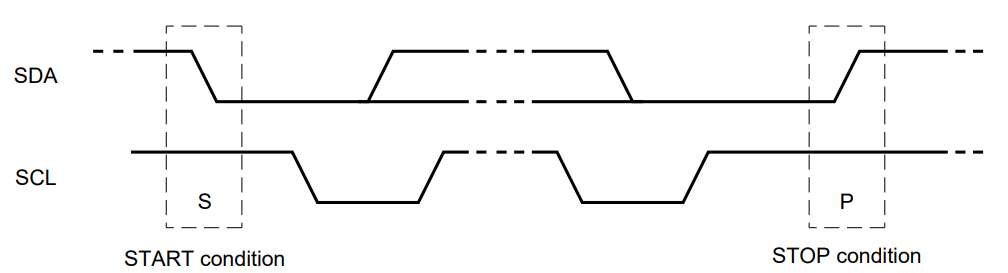
\includegraphics[scale=0.5]{start_stop_conditions}
\end{center}
One data bit is transferred during each clock pulse of the SCL, the data on the SDA line must remain stable duriong the high period of the clock pulse
as changes in the data line at this time will be interpreted as control signals (START or STOP). Any number of data bytes can be transferred between
ther START and STOP conditions. Data is transferred Most Significant Bit first.

\begin{center}
    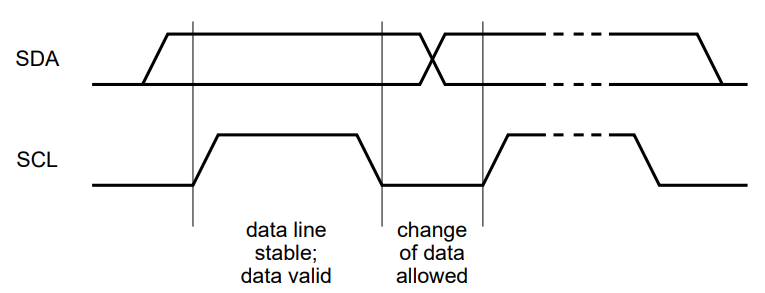
\includegraphics[scale=0.5]{bit_transfer}
\end{center}
Each byte of data is followed by one ACK (acknowledge) bit from the receiver to signal thath the byte was successfully received. Before the receiver can send an ACK 
de transmitter must realease the SDA line. To send an ACK bit the receiver pulls down the SDA after receiving the last bit so the line is stable low during the high 
fase of the ACK clock period. When SDA line remains high after receiving the last bit, this is interpreted as a NACK (not acknowledge)

\begin{center}
    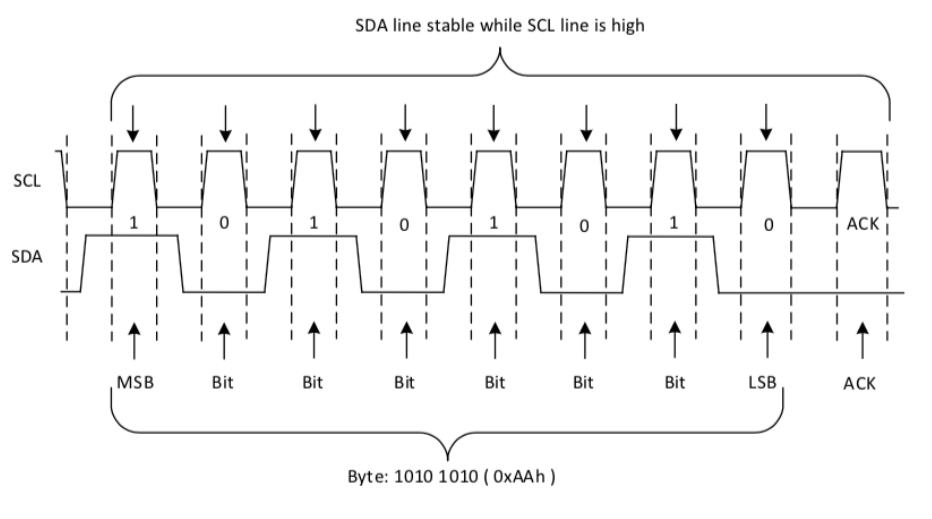
\includegraphics[scale=0.5]{byte_transmission}
\end{center}

The procedure to write on the bus is the following:
\begin{itemize}
    \item The master sends a START condition with the slave's address followed by the R/W bit set to 0
    \item The slave sends the acknowledge bit 
    \item The master sends the register address of the register it whishes to write to 
    \item The slave acknowledges the register address
    \item The master starts sending the register data to the slave 
    \item The master terminates the transmission with a STOP condition
\end{itemize}

\begin{center}
    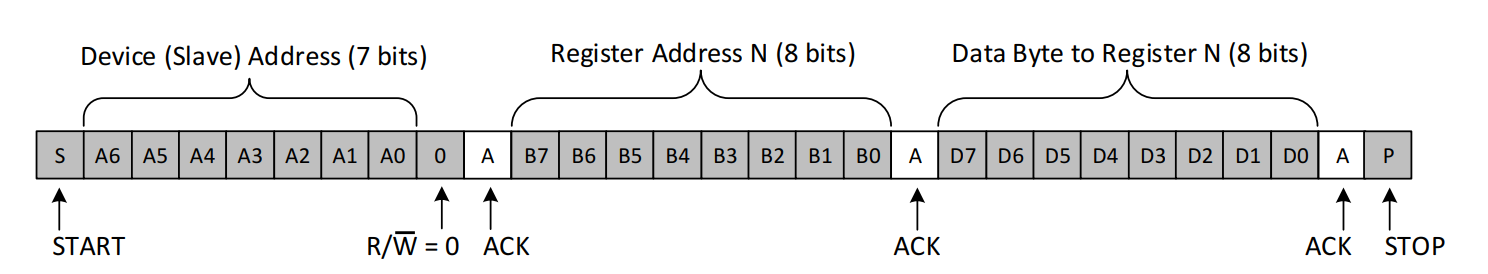
\includegraphics[scale=0.4]{write_procedure}
\end{center}

\subsubsection{LCD connection}
The following table describes the connections between the LCD 1602 and the PCF8574AT 

\begin{center}
    \begin{tabular}{|c|c|} 
        \hline
        PCF8574AT & LCD 1602 \\
        \hline
        P0 & RS \\
        P1 & RW \\
        P2 & E \\
        P3 & Backlight \\
        P4 & D4 \\
        P5 & D5 \\
        P6 & D6 \\
        P7 & D7 \\
        \hline
    \end{tabular}
\end{center}

In order to set the LCD 1602 to 4 bit mode it is necessary to send the following command 

\begin{center}
    \begin{tabular}{|c|c|c|c|c|c|c|c|c|} 
        \hline
        & D7 & D6 & D5 & D4 & Backlight & E & R/W & RS \\
        \hline
        2C & 0 & 0 & 1 & 0 & 1 & 1 & 0 & 0 \\
        28 & 0 & 0 & 1 & 0 & 1 & 0 & 0 & 0 \\
        \hline
    \end{tabular}
\end{center}

Now is possible to send a command signal or a data signal according to the following tables

\begin{center}
    \begin{tabular}{|c|c|c|c|c|c|c|c|c|} 
        \hline
        & D7 & D6 & D5 & D4 & Backlight & E & R/W & RS \\
        \hline
        MSB\_CMD C & B7 & B6 & B5 & B4 & 1 & 1 & 0 & 0 \\
        MSB\_CMD 8 & B7 & B6 & B5 & B4 & 1 & 0 & 0 & 0 \\
        LSB\_CMD C & B3 & B2 & B1 & B0 & 1 & 1 & 0 & 0 \\
        LSB\_CMD 8 & B3 & B2 & B1 & B0 & 1 & 0 & 0 & 0 \\
        \hline
    \end{tabular}
\end{center}

\begin{center}
    \begin{tabular}{|c|c|c|c|c|c|c|c|c|} 
        \hline
        & D7 & D6 & D5 & D4 & Backlight & E & R/W & RS \\
        \hline
        MSB\_DATA D & B7 & B6 & B5 & B4 & 1 & 1 & 0 & 1 \\
        MSB\_DATA 9 & B7 & B6 & B5 & B4 & 1 & 0 & 0 & 1 \\
        LSB\_DATA D & B3 & B2 & B1 & B0 & 1 & 1 & 0 & 1 \\
        LSB\_DATA 9 & B3 & B2 & B1 & B0 & 1 & 0 & 0 & 1 \\
        \hline
    \end{tabular}
\end{center}


\subsection{GPIO wiring diagram}

\begin{center}
    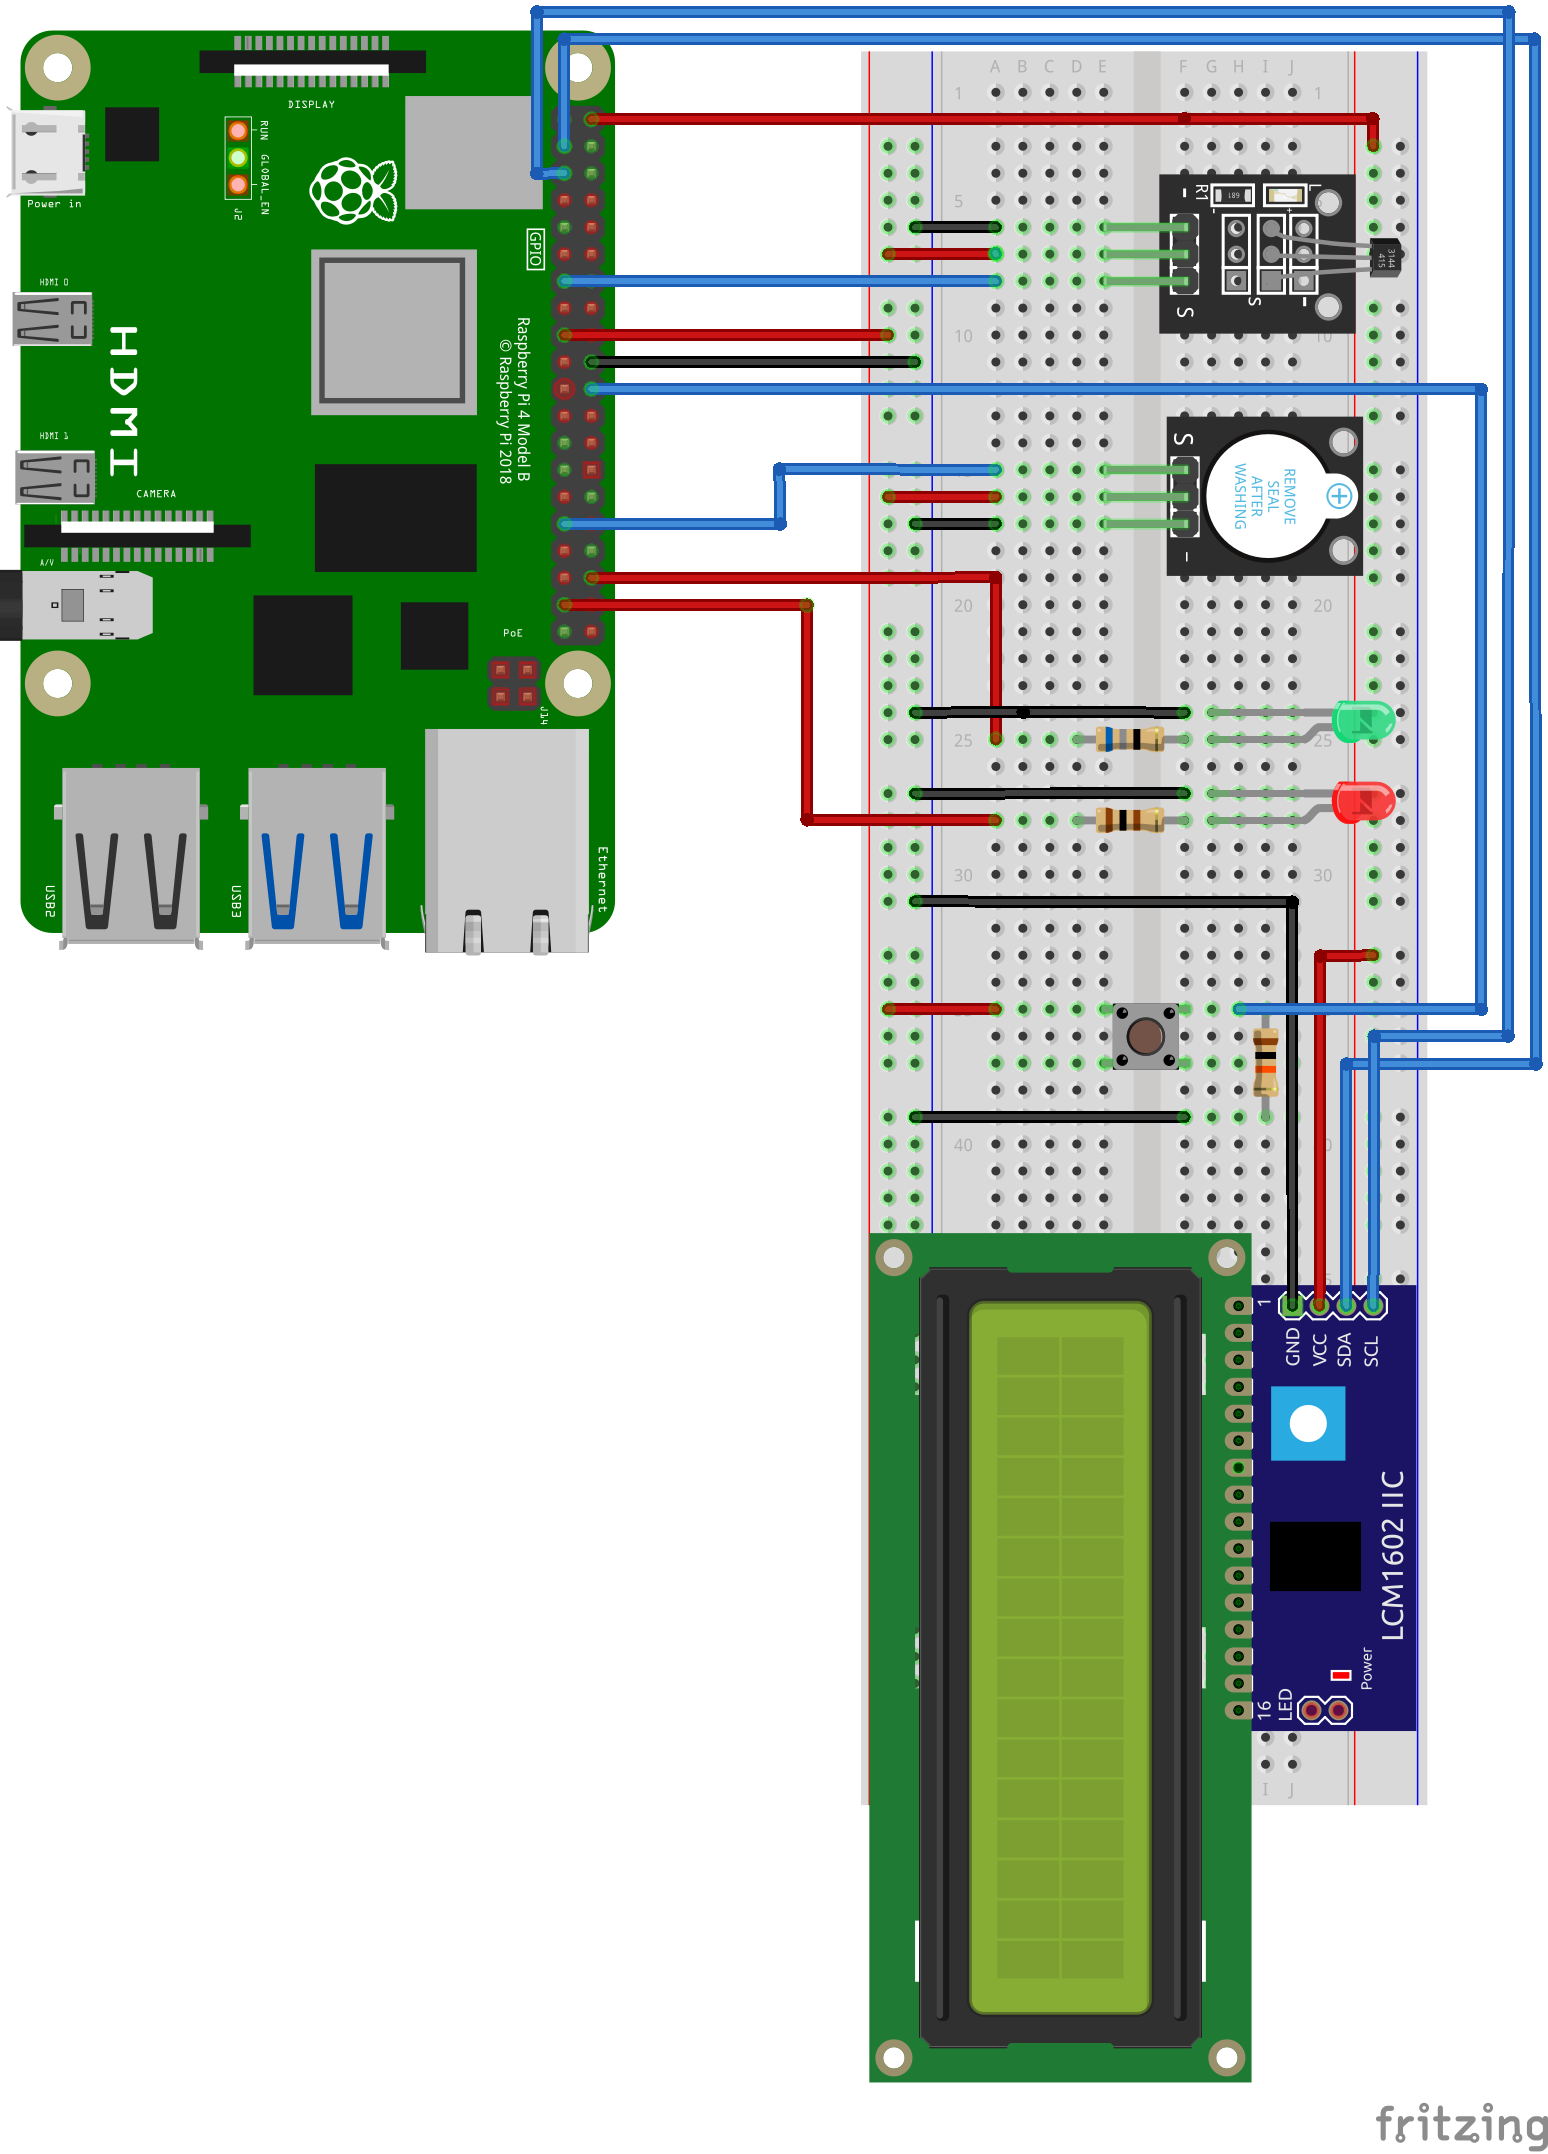
\includegraphics[scale=0.9]{breadboard}
\end{center}

\newpage
The following table is the GPIO wiring diagram.

\begin{center}
    \begin{tabular}{ |c|c|c| } 
        \hline
        GPIO & Function & Connection \\
        \hline
        2 & SDA & SDA (I/O expander) \\
        3 & SCL & SCL (I/O expander) \\
        6 & Output & S (Buzzer) \\
        16 & Output & Anode (Green LED) \\
        25 & Input & Button \\
        26 & Output & Anode (Red LED) \\
        27 & Input & S (Hall sensor) \\
        5V & Power & VCC (I/O expander) \\
        3V3 & Power & Breadboard \\
        Ground & Ground & Breadboard \\
        \hline
    \end{tabular}
\end{center}

\section{Environment}

\subsection{pijForthos}

\subsection{Minicom, Picocom}

\section{Software}

\section{References}

\begin{itemize}
    \item raspberrypi.com/products/raspberry-pi-4-model-b/specifications
    \item cdn.shopify.com/s/files/1/1509/1638/files/FT232-AZ\_Adapter\_Datenblatt\_AZ-Delivery-
    \\\_Vertriebs\_GmbH.pdf
    \item cdn.shopify.com/s/files/1/1509/1638/files/Hall\_Sensor\_Modul\_Digital\_Datenblatt.pdf
    \item cdn.shopify.com/s/files/1/1509/1638/files/KY-012\_Buzzer\_Modul\_Aktiv\_Datenblatt-
    \\\_AZ-Delivery\_Vertriebs\_GmbH.pdf
    \item wiki.52pi.com/index.php?title=Z-0234
    \item msb-co.ir/wp-content/uploads/2021/10/eone-1602a1.pdf
    \item nxp.com/docs/en/data-sheet/PCF8574\_PCF8574A.pdf
    \item ti.com/lit/an/slva704/slva704.pdf
\end{itemize}



\end{document}